\documentclass[11pt, a4paper]{article}

\usepackage{amsmath}
\usepackage{amsfonts}
\usepackage{graphicx}
\usepackage[export]{adjustbox}
\usepackage{hyperref}
\usepackage{fullpage}
\usepackage{caption}
\usepackage{listings}
\usepackage[dvipsnames]{xcolor}
\usepackage{gensymb}
\hypersetup{
    bookmarks=true,         % show bookmarks bar?
    unicode=false,          % non-Latin characters in Acrobat’s bookmarks
    pdftoolbar=true,        % show Acrobat’s toolbar?
    pdfmenubar=true,        % show Acrobat’s menu?
    pdffitwindow=false,     % window fit to page when opened
    pdfstartview={FitH},    % fits the width of the page to the window
    pdftitle={My title},    % title
    pdfauthor={Author},     % author
    pdfsubject={Subject},   % subject of the document
    pdfcreator={Creator},   % creator of the document
    pdfproducer={Producer}, % producer of the document
    pdfkeywords={keyword1, key2, key3}, % list of keywords
    pdfnewwindow=true,      % links in new PDF window
    colorlinks=true,       % false: boxed links; true: colored links
    linkcolor=Blue,          % color of internal links (change box color with linkbordercolor)
    citecolor=green,        % color of links to bibliography
    filecolor=magenta,      % color of file links
    urlcolor=red           % color of external links
}

\title{MAAS - Assignment-02\\
Proposed Architecture for \\Flying Saucers Bakery Project}
\author{Sushant Vijay Chavan\\Ahmed Faisal Abdelrahman\\Abanoub Abdelmalak}
\date{\today}

\begin{document}
\maketitle
\newpage
%\tableofcontents{}
\newpage

\section{The Architecture}
\begin{figure}[h!]
	\centering
	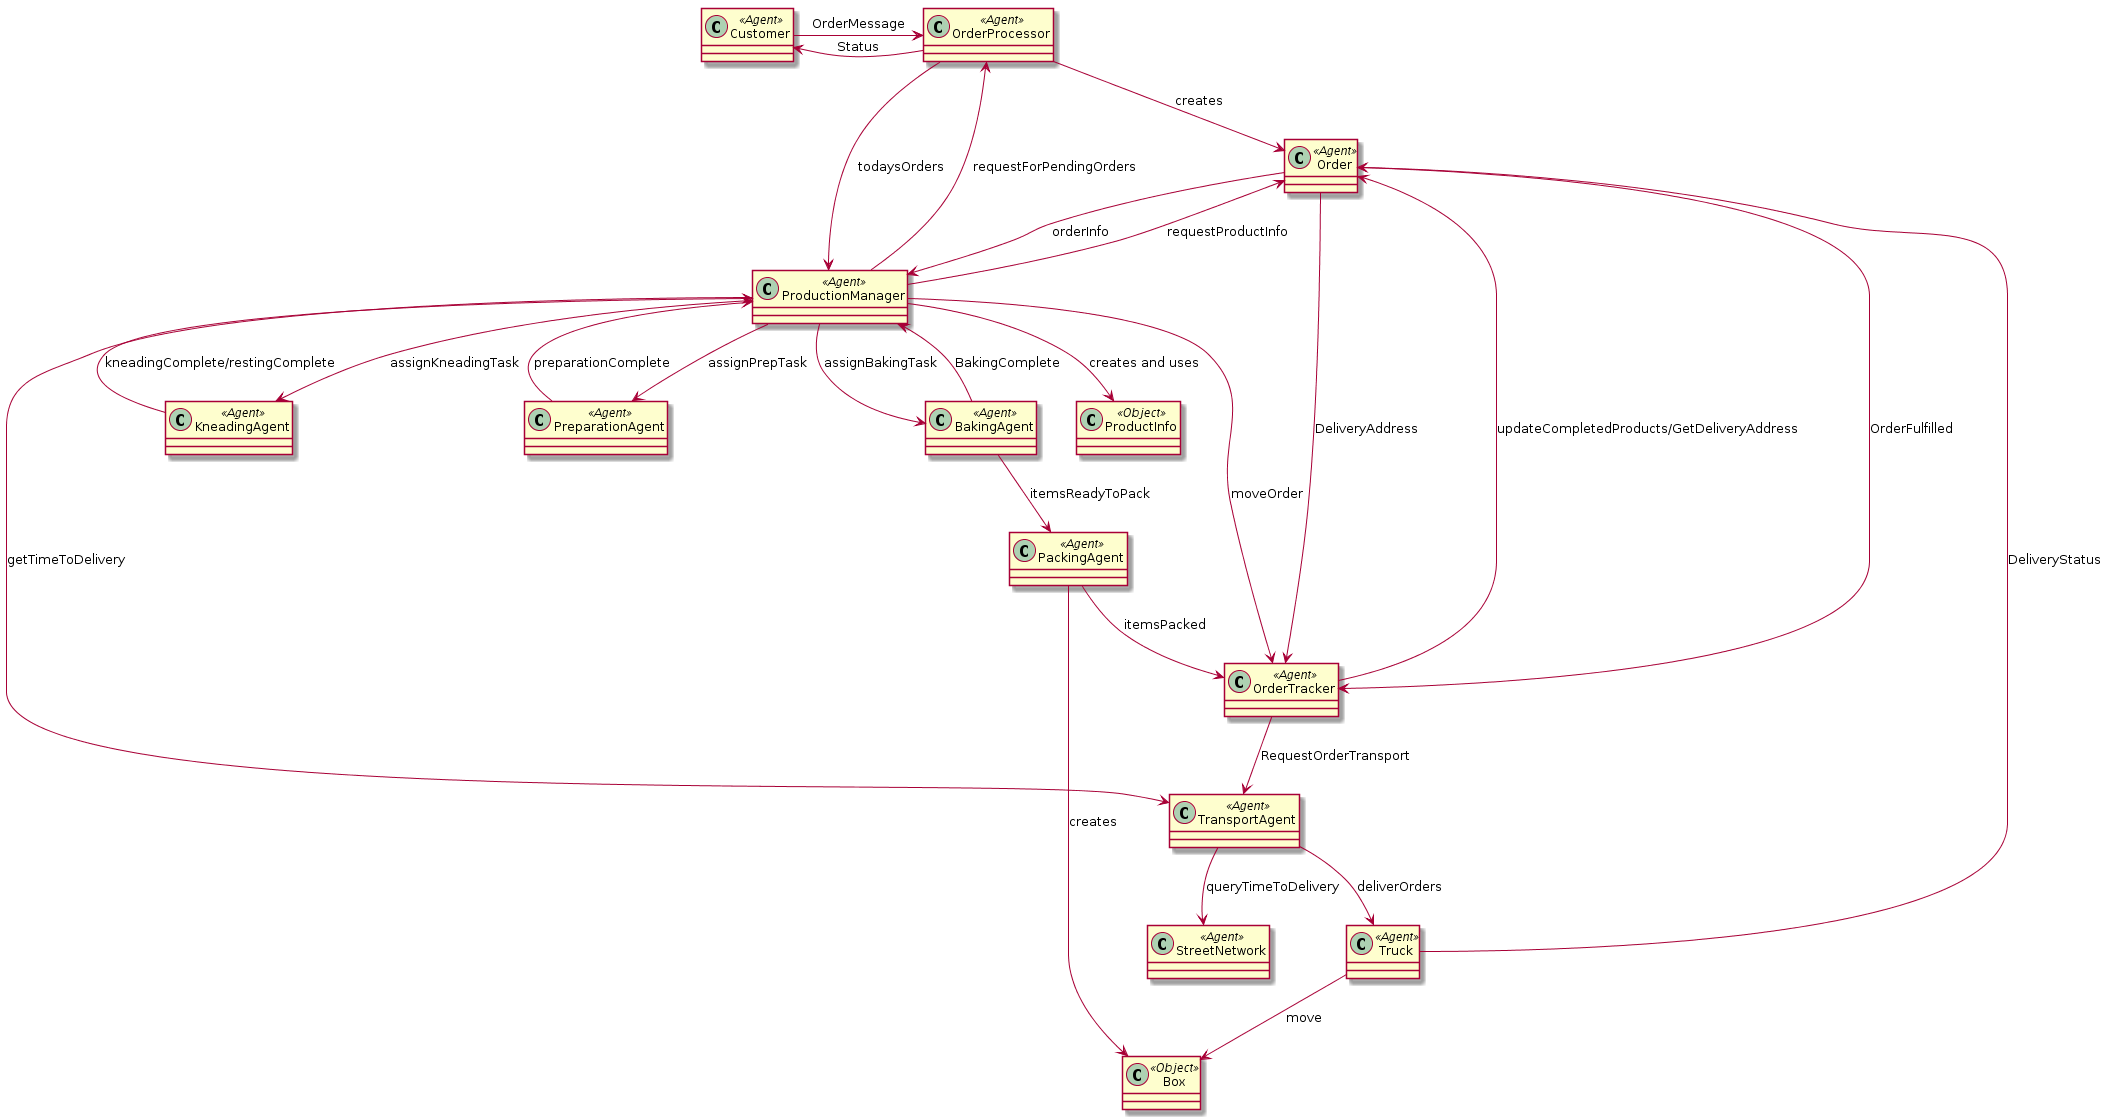
\includegraphics[angle=90, scale=0.385]{../Bakery.png}
	\caption{Architecture diagram}
	\label{Architecture diagram}
\end{figure}
The above figure \ref{Architecture diagram} outlines the overall architecture for the Flying Saucers Bakery project. The tags  above each of the components describe if the component is an object or an agent. The links between the components, represent the messages exchanged between the components. A detailed description of these messages can be looked up in the \textit{Messages.md} file.

\section{Agent Definitions}

The below table  lists out the details of each of the component that are a part of the architecture diagram.
\begin{table}[h!]
\centering
\begin{tabular}{|c|c|c|c|c|}
\hline
\textbf{Component}                                            & \textbf{\begin{tabular}[c]{@{}c@{}}Agent/\\ Object\end{tabular}} & \textbf{\begin{tabular}[c]{@{}c@{}}Static/\\ Dynamic\end{tabular}} & Stage                                                                      & Description                                                                                                                                                                       \\ \hline
Customer                                                      & Agent                                                            & Dynamic                                                            & Ordering                                                                   & Places the order for a set of items                                                                                                                                               \\ \hline
Order                                                         & Agent                                                            & Dynamic                                                            & \begin{tabular}[c]{@{}c@{}}Ordering/\\ Production/\\ Delivery\end{tabular} & \begin{tabular}[c]{@{}c@{}}Keeps track of a customer's request\\ for list of products at a given date\end{tabular}                                                                \\ \hline
Truck                                                         & Agent                                                            & Static                                                             & Delivery                                                                   & Delivers packed boxes that fulfill orders                                                                                                                                         \\ \hline
StreetNetwork                                                 & Agent                                                            & Static                                                             & Delivery                                                                   & \begin{tabular}[c]{@{}c@{}}Maintains a network of customer\\ and bakery locations\end{tabular}                                                                                    \\ \hline
\begin{tabular}[c]{@{}c@{}}Order-\\ Processor\end{tabular}    & Agent                                                            & Static                                                             & Order                                                                      & \begin{tabular}[c]{@{}c@{}}Receives and maintains the orders\\ until they are picked up for production\end{tabular}                                                               \\ \hline
\begin{tabular}[c]{@{}c@{}}Production-\\ Manager\end{tabular} & Agent                                                            & Static                                                             & Production                                                                 & \begin{tabular}[c]{@{}c@{}}Schedules and synchronizes the \\ activities of the rest of the agents\\ in the production stage\end{tabular}                                          \\ \hline
\begin{tabular}[c]{@{}c@{}}Kneading-\\ Agent\end{tabular}     & Agent                                                            & Static                                                             & Production                                                                 & \begin{tabular}[c]{@{}c@{}}Responsible for kneading\\ the dough and its resting time\end{tabular}                                                                                 \\ \hline
\begin{tabular}[c]{@{}c@{}}Preparation-\\ Agent\end{tabular}  & Agent                                                            & Static                                                             & Production                                                                 & \begin{tabular}[c]{@{}c@{}}Responsible for preparing \\ a given batch of items\end{tabular}                                                                                       \\ \hline
BakingAgent                                                   & Agent                                                            & Static                                                             & Production                                                                 & \begin{tabular}[c]{@{}c@{}}Responsible for maintaining the ovens\\  including making time and time to cool the baked \\ products and time to cool the baked products\end{tabular} \\ \hline
OrderTracker                                                  & Agent                                                            & Static                                                             & \begin{tabular}[c]{@{}c@{}}Production/\\ Delivery\end{tabular}             & \begin{tabular}[c]{@{}c@{}}Responsible for notifying the order \\ about their partial fulfillment\end{tabular}                                                                    \\ \hline
PackingAgent                                                  & Agent                                                            & Static                                                             & Production                                                                 & \begin{tabular}[c]{@{}c@{}}Packs the baked items into boxes when \\ they are cooled down\end{tabular}                                                                             \\ \hline
TransportAgent                                                & Agent                                                            & Static                                                             & Delivery                                                                   & \begin{tabular}[c]{@{}c@{}}Schedules the delivery of completed orders\\ by dividing them among truck agents\end{tabular}                                                          \\ \hline
ProductInfo                                                   & Object                                                           & Static                                                             & -                                                                          & \begin{tabular}[c]{@{}c@{}}Contains the details of the products\\ (e.g. time to bake, number of items in box)\end{tabular}                                                        \\ \hline
Box                                                           & Object                                                           & Dynamic                                                            & -                                                                          & \begin{tabular}[c]{@{}c@{}}Contains the type and quantity of \\ products packed in it\end{tabular}                                                                                \\ \hline
\end{tabular}
\label{Agent Definition}
\caption{Agent Definitions}
\end{table}

\newpage
\section{Aggregation of order data}

The OrderProcessor maintains a database of all the orders that have been received from customers, indexed by delivery date. The ProductionManager requests the OrderProcessor for the orders that are due for the day. It sorts the orders according to their delivery time and picks them in that order for production. If some agents are still free (e.g. to bake or prepare more items), the ProductionManager also schedules products to be prepared from the next order in the queue and so on.

\end{document}\grid
